The version of PMCLP where the facilities are ellipses that can be freely rotated was first introduced in \cite{andreta} where an exact and a heuristic method were developed for it. In comparison with MCE, this problem introduces a new variable that is responsible for determining the angle of rotation of every ellipse, making MCER a more challenging problem. We propose an algorithm for MCER which is able to obtain optimal solutions for every instance proposed in \cite{andreta} including the ones its exact method could not, and its heuristic obtained non-optimal ones.

%To make the text more clear, we introduce an equivalence relation for the set of solutions of MCER, and also a order relation making the set of solutions partially ordered.

Given an instance of the one-facility MCER, then given a solution $Q$ for it, with $|\Pp \cap E(q, \theta)| \ge 2$, if we rotate the coordinate system by $-\theta$, and use the result given by \autoref{lema:mce} for an axis-parallel ellipse, we can conclude that another solution $Q'$ exists, such that $Q' \succ Q$ and $|\Pp \cap \partial E(q', \theta)| \ge 2$. That is, given a solution for the one-facility MCER, we can obtain another one that covers the same points (possibly more) and the ellipse contains two demand points.

Next, we define a new notation that helps us characterize angles which given an ellipse rotated by it and two points, it is possible to find a center for the ellipse, such that it contains both points.

\begin{definition}\label{def:feasible_angle}
	Let $E$ be the coverage region of an ellipse and $u, v \in \R^2$. An angle $\theta \in [0, \pi)$ is said to be $(E, u, v)$-feasible if there is $q \in \R^2$ such that $\{u, v\} \subset \partial E(q, \theta)$.
	In addition to that, the set of $(E, u, v)$-feasible angles is referred to as 
	
	\begin{equation*}
	\Phi(u, v) := \{\theta \in [0, \pi) : \theta \textnormal{ is a } (E,u,v)\textnormal{-feasible angle}\}.
	\end{equation*}
	%We also define $\tilde{\Phi}_j(u,v)$ as the angle which makes $E_j$'s major-axis be parallel to the line that passes through $u$ and $v$. Note that if $\Phi_j(u,v) \neq \emptyset$, then $\tilde{\Phi}_j(u,v) \in \Phi_j(u,v)$ as the longest segment that crosses an ellipse is its major-axis.
\end{definition}

%%%%% TODO: TERMINEI DE REVISAR AKI.

\begin{figure}[H]
	\centering
	\includegraphics[scale=.22]{figures/feasible-angle2}
	\caption{The solid border ellipses are rotated by a $(E, u,v)$-feasible angle, while the ellipse with a dashed border is rotated by a not $(E, u, v)$-feasible angle.}
	\label{fig:feasible-angle}
\end{figure}

For any $x\in\R^2$, we denote by $\angle x\in [0, \pi)$ the minimal angle between $x$ and the vector $(1, 0)$. If $\Phi(u,v)\neq\emptyset$, then $\angle(u-v)\in  \Phi(u,v)$ as $\angle(u-v)$ is the angle that makes the ellipse's major-axis, the longest segment crossing an ellipse, be parallel to the line that passes through $u$ and $v$.

Next we open a parenthesis to discuss the problem of deciding for what angles of rotation it is possible to find a center for an ellipse, so it contains two given points. We give the result for two points that have the same $y$-coordinate, but this can be generalized.

\begin{lem}\label{lema:l-function}
	Given an instance of the one-facility MCER, if $u, v \in \Pp$ have the same $y$-coordinate and $||u-v||_2 \le 2a$, then $\Phi(u,v) = [0, \alpha] \cup [\pi - \alpha, \pi)$, for some $\alpha \in [0, \pi/2]$.
\end{lem}

\begin{proof}
	
	Consider an axis-parallel ellipse with shape parameters $(a, b)\in\R^2_{>0}$ centered at the origin, and a line represented by the equation $y=mx+c$, with $m, c\in \R$. Suppose that this line intersects the ellipse at least at one point. By plugging the line's equation into $x^2/a^2+y^2/b^2=1$, it is possible to obtain the distance between the intersection points. The final expression is given by
	\begin{equation*}\label{eq:dist_line_ellipse}
	D(m, c)=\dfrac{\sqrt{(a^2m^2+b^2-c^2)(4a^2b^2(1+m^2))}}{(a^2m^2+b^2)},
	\end{equation*}
	with $D : \R^2 \mapsto \R_{\ge0}$ being a function of the line parameters $(m, c)$.
	If $D(m, c) = ||u-v||_2$, then there exist $q_1, q_2 \in \R^2$, such that $\{u, v\} \subset \partial E(q_1, \tan{m})$ and $\{u, v\} \subset \partial E(q_2, \pi-\tan{m})$. It is also possible to see that, when $m$ is fixed, $D(m, c)^2$ is a parabola, and that $D(m, c)$ is maximized at $c=0$.  
	Following that, we define a function $L:\R\mapsto\R$ as
	
	\begin{equation*}
	L(m):= D(m, 0)^2 = \dfrac{(a^2m^2+b^2)(4a^2b^2(1+m^2))}{(a^2m^2+b^2)^2},
	\end{equation*}
	which describes the maximum distance between points of an ellipse-line intersection considering all lines with $m$ angular coefficient. From that, if $L(m) \ge ||v-u||_2^2$, then there exist $q_1, q_2\in\R^2$, such that $\{u, v\} \subset \partial E(q_1, \tan{m})$, and $\{u, v\} \subset \partial E(q_2, \pi-\tan{m})$.
	
	It is possible, by calculating the derivatives, to conclude that $L$ has its maximum at $m=0$, is increasing in $(-\infty, 0]$, is decreasing in $[0, \infty)$, and attains every value in the interval $(4b^2, 4a^2]$. Notice that $L$ never hits $4b^2$ because that is the distance between the intersection of the ellipse with a vertical line.
	%In \autoref{fig:L-function-plot}, an example of function $L$ is shown with $(a, b) = (2, 1)$.
	
	If $\inf{L} \ge ||u-v||_2^2$, then $\Phi(u,v) = [0, \pi)$.
	Otherwise, let $\beta \in \R$, $\beta \ge 0$, such that $L(\beta) = ||u-v||_2^2$, then as $m>\beta$, we have $L(m) < ||u-v||_2^2$, which means that it is impossible to make the ellipse contain $u$, and $v$.
	As $L$ is an even function, the same can be said for $m < \beta$. Therefore, we conclude that $\Phi(u,v)=[0, \tan(\beta)] \cup [\pi-\tan(\beta), \pi)$.
\end{proof}
%\begin{figure}[H]
%	\centering
%	\includegraphics[scale=.4]{../tex/figures/L-function-plot}
%	\caption{Plot of function $L$ in the interval $[-7, 7]$.}
%	\label{fig:L-function-plot}
%\end{figure}



%%% Fim L function

Following that, we introduce a lemma that is responsible for connecting the developments of this chapter with the results of Section~\ref{section:e3p}.
This lemma makes it possible to describe a type of solution which, for sure, is part of the equivalence class of any optimal solution.
It states that, for any ellipse that covers more than two points in a given optimal solution, an equivalent solution exists with at least one of the two properties:
\begin{itemize}
	\item The ellipse contains at least three points.
	\item The ellipse contains two points for any feasible angle.
\end{itemize}


\begin{lem}\label{lema:3pnts}
	Let $Q^*$ be a solution of the one-facility MCER, such that $|\Pp \cap E(q^*, \theta^*)|\ge2$.
	If for all $\bar{Q} \succ Q^*$, $|\Pp \cap \partial E(\bar{q}, \bar{\theta})| < 3$, then there exists $\{u, v\} \subset \Pp \cap E(q^*, \theta^*)$, such that for all $\theta\in \Phi(u,v)$ there exists $q \in \R^2$, such that $(q, \theta)$ is equivalent to $Q^*$.
\end{lem}

\begin{proof}
	According to \autoref{lema:mce}, there exists $\{u, v\} \subset \Pp \cap E(q^*, \theta^*)$, such that $Q' \succ Q^*$ exists, and $\{u, v\} \subset \partial E(q', \theta^*)$. Therefore, $\theta^*\in\Phi(u,v)$.
	
	Suppose that $u$ and $v$ have the same $y$-coordinate (if they do not, a rotation can be applied to make them do). Then, by \autoref{lema:l-function}, $\Phi(u,v)=[0, \alpha] \cup [\pi-\alpha, \pi)$, for some $\alpha \in [0, \pi/2]$. Then, if we rotate the coordinate system by $\pi-\alpha$, we obtain $\Phi(u,v)=[0, 2\alpha]$.
	
	With this result in hand, we can use a continuity argument to complete our proof as follows.
	Let $\delta : \Phi(u,v) \mapsto \R^2$ be a continuous function which takes an angle $\theta\in\Phi(u,v)$ and returns a center, such that $\{u,v\} \subset \partial E(\delta(\theta), \theta)$, and, from solution $Q'$, $\delta(\theta') = q'$. Notice that, in general, for any angle in $\Phi(u,v)$, there are two possible centers that make $\{u,v\} \subset \partial E(\delta(\theta), \theta)$ (see \autoref{fig:feasible-angle} for an example), however, imposing $\delta(\theta') = q'$ makes $\delta$ be a well-defined continuous function. This is shown in \autoref{fig:lema-3-points} where $\delta$ is plotted for the whole interval $\Phi(u,v)$.
	
	Let $w\in \Pp \setminus \{u,v\}$, then we define $f_w  : [0, \pi) \mapsto \R_{\ge0}$ to be a function that takes an angle of rotation $\theta$ and returns the elliptical distance $||\cdot||_{a,b,\theta}$ to the center $\delta(\theta)$; that is $f_w(\theta)=||w-\delta(\theta)||_{a,b,\theta}$.
	We have that if $w \in \Pp \cap E(q^*, \theta^*)$, then $f_w(\theta^*) \le 1$; and if $w \not\in \Pp \cap E(q^*, \theta^*)$, then $f_w(\theta^*) > 1$.
	
	Therefore, if there exists $\theta\in\Phi(u,v)$, such that for all $q\in\R^2$, $(q, \theta)$ is not equivalent to $Q^*$, then there exists either $w \in \Pp \cap E(q^*, \theta^*)$, with $f_w(\theta)>1$, or $w \not\in \Pp \cap E(q^*, \theta^*)$, with $f_w(\theta)\le 1$. Because $f_w$ is continuous, there exists $\bar{\theta}\in\Phi(u,v)$, such that $f_w(\bar{\theta})=1$, implying that $|\Pp \cap \partial E(\delta(\bar{\theta}), \bar{\theta})| \ge 3$.
\end{proof}

In \autoref{fig:lema-3-points}, a visualization of \autoref{lema:3pnts} is presented.
An initial solution is given by the dashed-border ellipse and its center, represented by a star point. From it, the continuous function $\delta$ is defined by moving the ellipse through the rotation angles in $\Phi(u,v)$ while maintaining $u, v$ on it. Six angles were chosen from $\Phi(u,v)$ to be shown in \autoref{fig:lema-3-points}, among those were $0$ and $\max\{\Phi(u,v)\}$; their corresponding ellipses are displayed with solid-line borders.
Consistently with \autoref{lema:3pnts}, the points in $\Pp \setminus \{u, v, w\}$ stay within the ellipse's cover for any angle of rotation, and, for point $w$, there exists an angle, such that it is on the ellipse, which is a solution of E3P.

\begin{figure}[H]
	\centering
	\includegraphics[scale=.7]{figures/lema-3-points}
	\caption{A visualization of \autoref{lema:3pnts}.}
	\label{fig:lema-3-points}
\end{figure}

\begin{definition}\label{def:Sj}
	Given an instance of MCER. Then, for all $j\in\{1, \dots, m\}$, we define the CLS of the $j$-th ellipse as $S_j = S_j^{(1)} \cup S_j^{(2)} \cup S_j^{(3)}$ with
	\begin{align*}
	S_j^{(1)} &= \bigcup_{u \in \Pp} \{(u, 0)\}\\
	S_j^{(2)} &= \bigcup_{\{u, v\} \subset \Pp} \{(q, \angle(u-v))\in \R^2\times[0, \pi): \{u,v\} \subset \partial E_j(q, \angle(u-v))\}\\
	S_j^{(3)} &= \bigcup_{\{u, v, w\} \subset \Pp} \{(q, \theta)\in \R^2\times[0, \pi): \{u, v, w\} \subset \partial E_j(q, \theta)\}.
	\end{align*}
\end{definition}

This definition breaks the construction of the CLS into three separated cases. The first one, $S_j^{(1)}$, represents solutions where the $j$-th ellipse covers only one point. The second one, $S_j^{(2)}$, takes into account solutions where the $j$-th ellipse covers at least two points, and no equivalent solution with three points on the ellipse exists. The last case, $S_j^{(3)}$, considers solutions where there exists an equivalent one with three points on the $j$-th ellipse. 

To compute $S_j^{(2)}$, we can observe that, given two points $u, v$, determining every $q\in\R^2$, such that $\{u,v\}\subset\partial E_j(q, \angle(u-v))$ can be transformed into the problem of determining the set $\partial E_j(u, \angle(u-v)) \cap \partial E_j(v, \angle(u-v))$, which, by \autoref{lema:e2p}, is composed of at most two points, which can be determined analytically. Therefore, we have that $S_j^{(2)}$ can be computed in $\bigO(n^2)$ operations.

To compute $S_j^{(3)}$, we have to call the algorithm described in Section~\ref{section:e3p} to determine every solution of E3P for every triplet of points in $\Pp$. Even though that algorithm is $\bigO(1)$, it has a high constant factor, thus skipping it, in practice, is a good suggestion.
Given three points and an ellipse with shape parameters $(a, b)$, the following two conditions are sufficient for E3P to have no solutions, and therefore, if any of them is true, we can skip calling the algorithm to determine every solution of E3P for that instance:
\begin{itemize}
	\item The maximum distance between any of the points is greater than $2a$;
	\item The triangle's area with vertices on these three points have area greater than $\frac{3\sqrt{3}}{4}\pi ab$, which can be proved to be the greatest area of an inscribed triangle in an ellipse with shape parameters $(a, b)$.
\end{itemize}

Overall, constructing every ellipse's CLS can be implemented to have a $\bigO(n^3)$ runtime complexity.
Following this, we introduce a theorem, which connects the results for MCER so far, to prove that the set of solutions constructed using the CLSs described by \autoref{def:Sj} contains an optimal solution.


\begin{thm}\label{th:mcer}
	Given an instance of MCER, let $\Omega$ be a set of solutions defined as 
	\begin{equation*}\label{eq:omega}
	\Omega = \{Q \in (\R^2\times[0, \pi))^m \colon (q_j, \theta_j) \in S_j \textnormal{ for all } j\in\{1, \dots, m\}\}.
	\end{equation*}
	Then there exists an optimal solution $Q^* \in \Omega$, and $|\Omega|\le n^{3m}$.
\end{thm}
\begin{proof}
	The first thing to notice is that $\Omega$ is defined as the combination of every possible solution from each CLS. To prove that it contains an optimal solution $Q^*$, we only need to prove that for all $j\in\{1, \dots, m\}$, there exists $(q_j, \theta_j)\in S_j$, such that $\Pp \cap E_j(q_j^*, \theta_j^*) \subset \Pp \cap E_j(q_j, \theta_j)$. To do that, we use \autoref{lema:3pnts} and break the possible optimal solutions into three cases.
	
	In the first case, we consider solutions where the $j$-th ellipse covers at most one point, that is, $|\Pp \cap E_j(q_j^*, \theta_j^*)|\le1$. It is possible to see that $S_j^{(1)}$ takes this possibility into account as it includes in $\Omega$ every solution that has an ellipse centered at a point from $\Pp$. From that, we can also conclude that $|S_j^{(1)}| = n$.
	
	In the second case, we consider solutions where the $j$-th ellipse covers at least two points, and there is no $Q' \succ Q^*$, such that $|\Pp \cap \partial E_j(q_j', \theta_j')| \ge 3$.
	This case is addressed by \autoref{lema:3pnts}, which states that there are equivalent solutions to $Q^*$ with two points $u, v \in \Pp \cap E_j(q_j^*, \theta_j^*)$ on the $j$-th ellipse for every $(E_j, u, v)$-feasible angle.
	As $\angle(u-v)$ is a $(E_j, u, v)$-feasible angle, we have that there exists $(q_j, \theta_j) \in S_j^{(2)}$, such that $\Pp \cap E_j(q_j, \theta_j) = \Pp \cap E_j(q_j^*, \theta_j^*)$.
	{\color{blue}Also from \autoref{lema:e2p}, we can arrive at the conclusion that $|S_j^{(2)}| \le 2\binom{n}{2}$.}
	
%	Moreover, as determining every $q\in\R^2$, such that $\{u,v\}\subset \partial E_j(q, \angle(u-v))$ can be transformed into the problem of determining the set $\partial E_j(u, \angle(u-v)) \cap \partial E_j(v, \angle(u-v))$, which, as discussed in \autoref{section:mce}, contains at most two points, we can conclude that $|S_j^{(2)}| \le 2 \binom{n}{2}$.
	
	For the last case, we are left with solutions where the $j$-th ellipse covers more than two points, and there exists an equivalent solution with three points on it. 
	As $S_j^{(3)}$ contains every center and angle of rotation that puts three points on the $j$-th ellipse, an equivalent solution for this case is present in the set of solutions $\Omega$. Also, by \autoref{lema:e3p} we can conclude that $|S_j^{(3)}| \le 6\binom{n}{3}$.
	
	Combining the three cases, as $S_j=S_j^{(1)}\cup S_j^{(2)} \cup S_j^{(3)}$, we get the following bound for $|S_j|$:
	\begin{eqnarray*}
		|S_j| &\le 6\binom{n}{3} + 2\binom{n}{2} + n &= n(n-1)(n-2) + n(n-1) + n\\
		|S_j| &\le 6\binom{n}{3} + 2\binom{n}{2} + n &= n((n-1)^2+1) \le n^3.
	\end{eqnarray*}	
	Therefore, we conclude that  $|\Omega| \le |S_1|\times \dots \times |S_m| \le n^{3m}$.
\end{proof}

Finally, we define \autoref{algoritmo:mcer}, which backtracks every possible combination of solutions considering the CLS of every ellipse.
As evaluating each solution can be implemented to take $\bigO(nm)$ operations, we have that \autoref{algoritmo:mcer} has a $\bigO(mn^{3m+1})$ runtime complexity.
In the next section, we describe some implementation details and improvements that, in practice, can lower the size of $S_j$ significantly, and also can make the backtracking process described in \autoref{algoritmo:mcer} skip many non-optimal solutions.

\begin{algorithm}
	\caption{Algorithm for MCER}\label{algoritmo:mcer}
	\begin{algorithmic}[1]
		\Require{A set of points $\Pp=\{p_1,\dots,p_n\}$, a list of weights $\Ww=\{w_1, \dots, w_n\}$, and a list of shape parameters $\Rr=\{(a_1, b_1), \dots, (a_m, b_m)\}$.}
		
		\Ensure{An optimal solution for the given instance of MCER.}
		
		\item[]
		\Procedure{$MCER$}{$\Pp, \Ww, \Rr$}
		\State \Return $MCER_{bt}(\Pp, \Ww, \Rr, 1)$
		\EndProcedure
		
		\item[]
		
		\Procedure{$MCER_{bt}$}{$Z, \Ww, \Rr, j$}
		%\If{$j = m+1$}
		%\State \Return $0$
		%\EndIf
		
		%\State $ans \gets 0$
		\State $(q_{j}^*,\theta_j*); \dots; (q_m^*, \theta_m^*) \gets (0,0); \dots; (0, 0)$ \Comment{Setting to $0$ as a default value.}
		
		%\State $S_j \gets \textnormal{CLS-MCER}(Z, a_j, b_j)$
		\State Let $S_j$ be the CLS for the $j$-th ellipse as defined in \autoref{def:Sj}
		
		\ForAll{$(q_j, \theta_j) \in S_j$}
		\State $Cov \gets \Pp \cap E_j(q_j, \theta_j)$
		
		\If{$j < |\Rr|$}
		\State $(q_{j+1},\theta_{j+1}); \dots; (q_m,\theta_m) \gets  MCER_{bt}(Z\setminus Cov, \Ww, \Rr, j+1)$
		\EndIf
		
		%\State $Cov \gets \bigcup_{k=j}^m \Pp \cap E_k(q_k, \theta_k)$
		\If {$w(\bigcup_{k=j}^m \Pp \cap E_k(q_k, \theta_k)) > w(\bigcup_{k=j}^m \Pp \cap E_k(q_k^*, \theta_k^*))$}
		%\State $ans \gets w(Cov)$
		%\State $((q_{j}^*,\theta_{j}^*); \dots; (q_m^*, \theta_m^*)) \gets ((q_{j},\theta_{j}); \dots; (q_m, \theta_m))$
		
		\State $(q_{j}^*,\theta_j*); \dots; (q_m^*, \theta_m^*) \gets  (q_{j},\theta_{j}); \dots; (q_m,\theta_m) $
		\EndIf
		\EndFor
		
		\State \Return $(q_{j}^*,\theta_j*); \dots; (q_m^*, \theta_m^*)$
		\EndProcedure
	\end{algorithmic}
\end{algorithm}